% PREAMBLE
\documentclass{article}
\title{My journey to Blackwater}
\author {William Thorne}
\date{12.12.1997}
\usepackage{graphicx}
\usepackage{subcaption}
\usepackage{float}

% DOCUMENT
\begin{document}
\pagenumbering{gobble}
\maketitle
\newpage
\begin{figure}[!h]
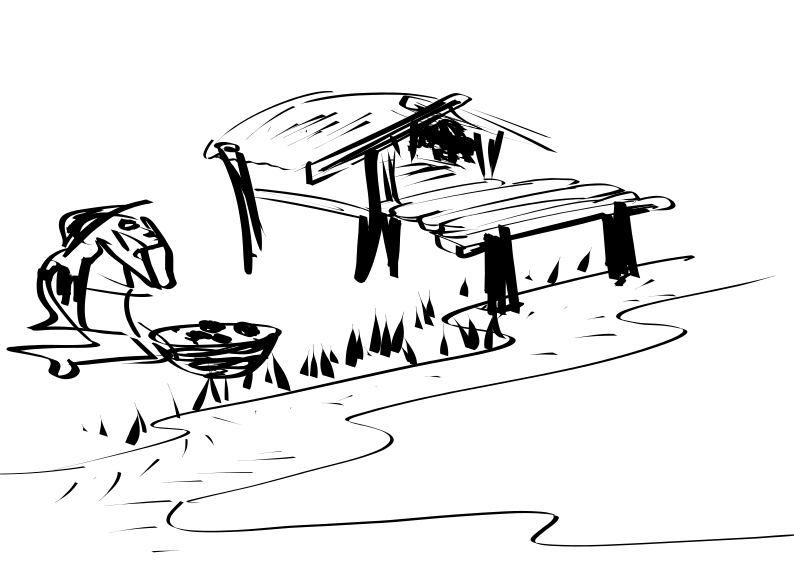
\includegraphics[width=\linewidth]{resources/blackwater.png}
\caption{Me at Blackwater, thankful for a basket of fruits.}
\label{fig:blackwater}
\end{figure}

In Figure \ref{fig:blackwater} you can see my highness William Thorne succumbing to nature at Blackwater. I had been walking for months and weeks and my feet were so happy to see sunlight again after they had been coming out of the black slimy water. 
\section{Pirate Flag Comparison}
However in the following I will ask you about an important question.
As you know Blackwater was and still is a city full of pirates. So in case you ever would like to visit it as well, what is your favourite pirates flag? In Figure \ref{fig:pflag-compare} you can dwell on the beauty of four different candidates for the new best pirate flag of the world!

\begin{figure}[H]
  \centering
   \begin{subfigure}[b]{0.3\linewidth}
    
\includegraphics[width=\linewidth]{resources/pirates1.png}
    \caption{First Choice.}
  \end{subfigure}
  \begin{subfigure}[b]{0.3\linewidth}
    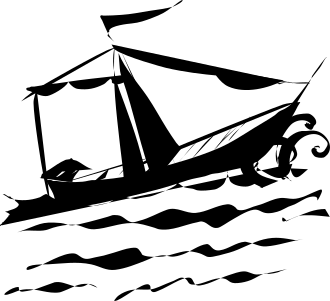
\includegraphics[width=\linewidth]{resources/pirates2.png}
    \caption{Second Choice. (Might better right?)}
  \end{subfigure}
  \begin{subfigure}[b]{0.4\linewidth}
    
\includegraphics[width=\linewidth]{resources/pirates3.png}
    \caption{Third Choice.}
  \end{subfigure}
  \begin{subfigure}[b]{0.4\linewidth}
    
\includegraphics[width=\linewidth]{resources/pirates4.png}
    \caption{Fourth Choice. (Pretty awesome right??)}
  \end{subfigure}
  \begin{subfigure}[b]{0.7\linewidth}
    
\includegraphics[width=\linewidth]{resources/pirates4.png}
    \caption{My own Choice.}
  \end{subfigure}

  \caption{Two different approaches to establish a new best pirate flag ever.}
  \label{fig:pflag-compare}
\end{figure}






\end{document}
